\documentclass{article}
\usepackage{paralist} % Used for the compactitem environment which makes bullet points with less
\begin{document}


\section{Deploy test environment}
Many security network and software analysis research start with preparing the test environment. The test environment is deployed in the most cases as the virtual network with configured hosts, routers, networks and all others resources including users account. The test environment could be deployed on the local computer by using the software for virtualization like the VirtualBox, VmWare Workstation and others or could be deployed on the remote server with installed hypervisor software like VMware vSphere Hypervisor (ESXi).          

The common way to create the developing environment is to do it manually. You have to download image of operation system, install it on the Virtual Machine, configure it, install necessary softwares. The developing environment is usually more complex just one virtual machine, so you have to do the same step several. In some cases you can just clone virtual machine, but you still have to do a lot of manual work.       
  
There are some software which can simplify the process of creating the developing/test environment. One of the them is Vagrant. Vagrant allows to create and configure lightweight, reproducible, and portable development environments. The configured environment could be reused. Vagrant project has the relative project which is called VagrantCloud. The project is hosted on the https://vagrantcloud.com. It is some kind of the catalog of prepared environments. The prepared developing environment is called box.  People could share with community their boxes. Everyone could find the appropriate environment and reuse it instead of configuring new one. Vagrant allows to deploy the environment into the local VirtualBox, VMware Workstation, Aamazon Web Service (AWS). It means researchers are quite free in using the platform. The features of the Vagrant are not bound only by running the environment. The application a lot of give capabilities including synchronizing between the host and guest machine, integration with Chef[*], Puppet[*] and other. Learn more on the official website http://www.vagrantup.com/ 

The process of creating the development/test environment can by simplify by cloud providers. Many cloud providers provide capability easy to install and run virtual machine with any operation systems, configure the network and many other features. The most popular is Amazon Web Service (AWS). AWS is Infrastructure-as-a-Service. AWS provides huge amount of service which could solve any problem.  You could combine any infrastructure service to create the certain development environment. I mentioned just AWS, but the market of cloud providers grows extremely so it is possible find any other. As Vagrant AWS also provide capability to save configuration of the development environment, distribute it and reuse.

But we are talking about the researches with security aspects. It means that results and the process of the research in the most cases must secret. In this case it is not possible to use public cloud providers. Here opensource communities come to help us. There si not sense to tell that opensource communities grow extremely. A lot of big IT companies invest into the opensource projects. Many of these opensource projects are widely spread. They are use everywhere. So it does not go past the cloud technologies. There several opensource cloud platform which could be used for creating own IaaS, PaaS and other. Some of them: OpenStack, OpenNebula,  OpenShift Origin and so on. So clouds become private. For us it means that we could create our test/development environments by using flexibility and capability of cloud services. But still there are some problems and overhead of creating the test/development environments. It could be solved by using the PaaS, but PaaS's are usually designed for specific task mostly for running the infrastructure for web applications in Java, PHP, Ruby and so on. No one does provide flexible platform as a service based on all functionality of infrastructure as a service. We would like to call it Platform as a Infrastructure (PaaI). Jeslastic[*] uses this definition for describing its service, but they include other meaning into this definition.     

        


\section{Simulation of users behaviors}
There is task to analyses the behavior of users to predict attacks or abnormal behavior. There are some algorithms for Attack Prediction based on Machine Learning [http://www.csjournals.com/IJCSC/PDF1-2/51..pdf]. The algorithms could be used for research purposes, in this task the big problem is lack of data. The customer do not want and can not provide Active Directory log files which contains information about user activities. We have to start research since writing the script for simulation user behaviors. 

The Scenario in our case is the description of the network infrastructure, information about users, and scenario of their behavior. To analysis user behaviors by predict algorithms we must have normal scenario and abnormal scenario.  
  
\subsection{Environment description}

Description of a network:
\begin{compactitem}
\item 4 computers.
\item Domain controller. 
\item Wiki Server.
\item DB server.
\end{compactitem}
Users: 
\begin{compactitem}
\item Petrov
\item Ivanov 
\item Smirnov
\item Admin
\end{compactitem}
     
\subsection{Normal scenario}
Figure 1. Usually ordinal users login to their computers. They do it several times per day. All users and admin have an access to Wiki, but Ivanov usually do not use it. Admin usually login to Domain Controller. Other users do not do it, because their do not have an access. Ivanov does not login to wiki, but he has an access. Others users do it. Ivanov sometimes login to DB Server. Others users do not do it, but they have an access.
\begin{figure}[ht!]
\centering
%[width=90mm]
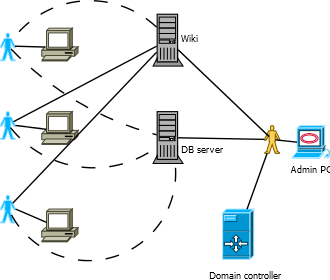
\includegraphics{scenario_normal.png}
\caption{Normal scenario}
\label{overflow}
\end{figure}

\subsection{Abnormal scenario}
Figure 2. Ivanov logged to wiki. He usually does not do it, but he has an access and other users do it every day. Petrov logged to DB server. He has an access, but according to the normal behavior only Ivanov uses the DB server. So it could be abnormal behavior.  

\begin{figure}[ht!]
\centering
%[width=90mm]
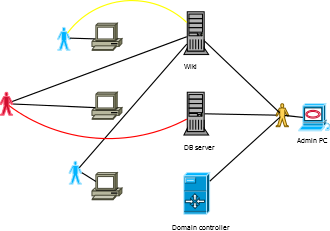
\includegraphics{scenario_abnormal.png}
\caption{Abnormal scenario}
\label{overflow}
\end{figure}

\subsection{Implementation}
The network is deployed and configured manually on the FutureSOC server with WMware ESXi. The script for the simulation users activities is written in Python with using additional libraries for connecting to Virtual Machines by VNC and making screenshots. There are 3 csv files for describing the whole scenario. The first of them (computers.csv) describe the the all computers which participate in the scenario. It contains the information about computer identifier, IP, port, VNC password and type of operation system(OS).
The second (scenarios.csv) describes the main user activity. The main user activity means the connection to the local computer. The files contains computer identifier to connect, username, password, session time, count of sessions and identifier of inner scenario.
The third (inner-scenarios.csv) describes the user activity after login to the local computer. For example, it could describe the connection to the wiki, the DB server or Domain Controller or even connection to another user computer.  
There are two sets of csv files. The first set is used to perform normal scenario and the second is used to perform abnormal scenario 	
accordingly. Normal scenario takes about 3,5 hours and abnormal scenario takes about 5,5 hours.
 
\end{document} 